\section{Data Curation}

% ============================================================
% Method
% Three-pillar structure:
%   1. Data Iteration Flywheel  (methodology)
%   2. Document Data Synthesis Engine  (tool for flywheel Stage 3 / Path B)
%   3. Dataset Preparation  (final training data composition)
% ============================================================

Our method centers on three pillars that jointly drive the construction of Infinity-Parser2. First, we propose a \textbf{data iteration flywheel} (Sec.~\ref{sec:flywheel}), a closed-loop methodology in which model evaluation, bad-case mining, data construction, and fine-tuning continuously reinforce one another. Second, to support the data construction step at scale, we develop a dedicated \textbf{document data synthesis engine} (Sec.~\ref{sec:synthesis}) that produces layout-faithful documents through a three-stage pipeline. Third, we describe the resulting \textbf{task-specific datasets} (Sec.~\ref{sec:dataset}) used to train the model across structure analysis, element recognition, and document reasoning tasks. In short, Sec.~\ref{sec:flywheel} formalizes \emph{how} data evolves with the model, Sec.~\ref{sec:synthesis} details \emph{what tool} produces this data at scale, and Sec.~\ref{sec:dataset} describes \emph{what data} the model is ultimately trained on.

% ============================================================
% Section 1: Data Iteration Flywheel
% ============================================================
\subsection{Data Iteration Flywheel}
\label{sec:flywheel}

\textbf{Overview.} Data quality and data construction strategy play a critical role in multimodal document understanding. While raw document data are abundant, transforming them into high-quality, task-relevant training data under limited annotation and compute budgets remains a major challenge. Static data pipelines, which fix the dataset before training begins, cannot respond to the model's evolving weaknesses and therefore tend to over-invest in already-mastered patterns while under-covering rare or difficult cases.

To address this, we propose a model-driven data iteration flywheel that tightly couples data construction with model behavior. Rather than statically defining sample importance, the flywheel dynamically estimates sample value based on the current model's inference results and iteratively refines the dataset.

As illustrated in Figure~\ref{fig:data_flywheel}, each turn of the flywheel comprises four stages:
(1) \emph{Model Evaluation and Bad-case Analysis},
(2) \emph{Data Collection and Mining},
(3) \emph{Model Annotation and Data Synthesis}, and
(4) \emph{Model Fine-tuning and Iteration}.
We describe the details of each stage in the following sections.

\begin{figure*}[htbp]
    \centering
    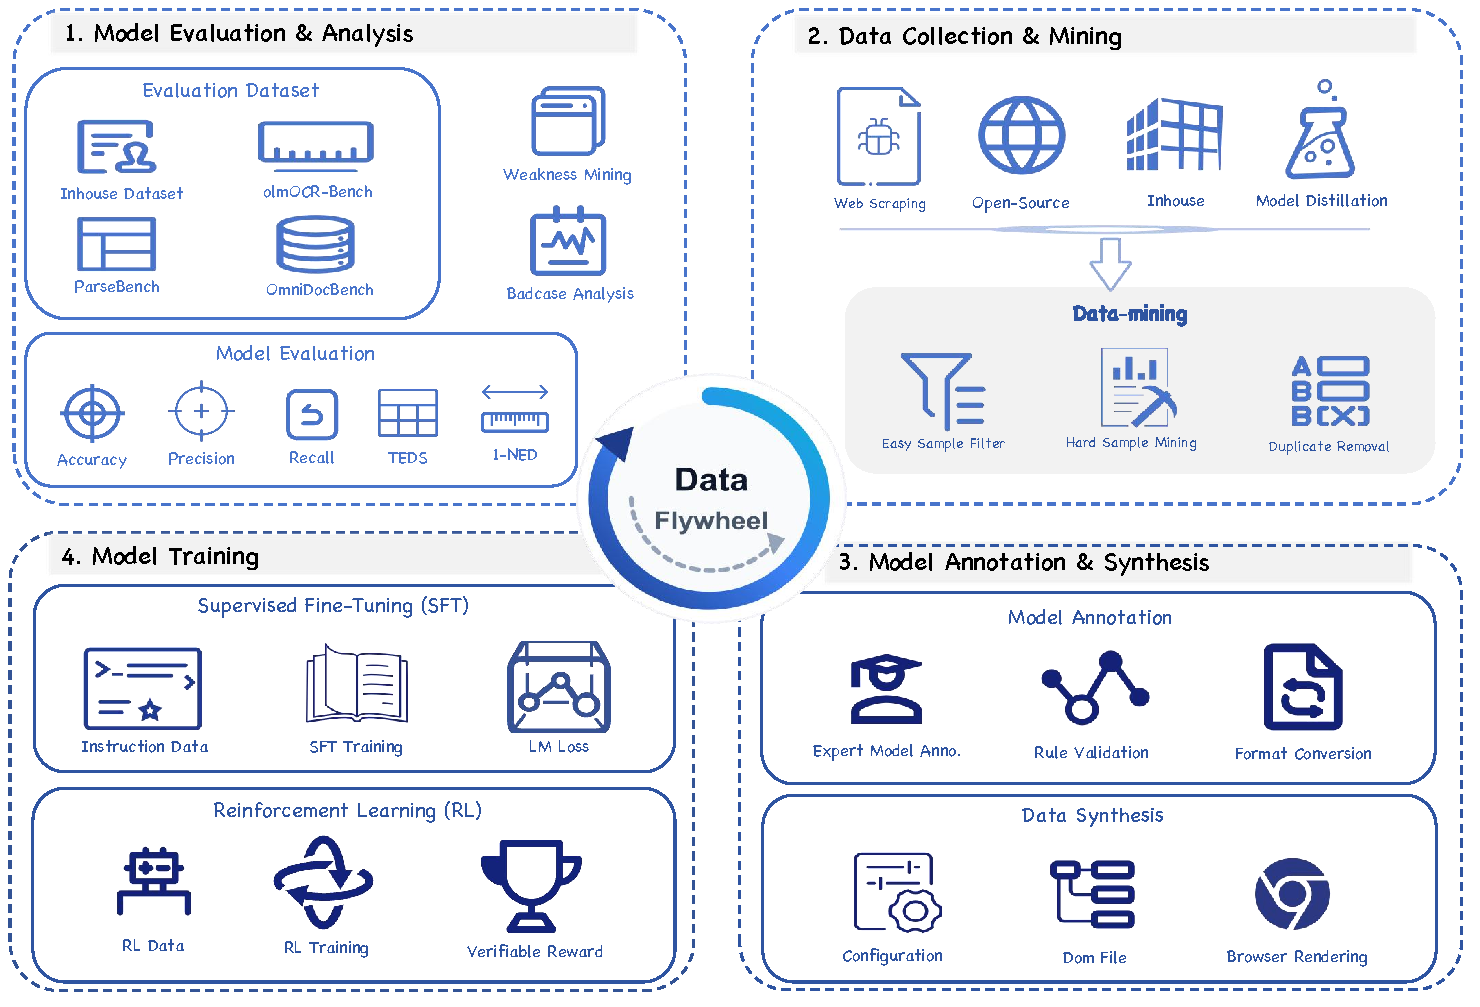
\includegraphics[width=\textwidth]{figures/data_flywheel_0605.pdf}
    \caption{Overall pipeline of our data iteration flywheel, a closed loop of four stages. Stage 1 evaluates the current model and consolidates its failures into a weakness taxonomy, Stage 2 collects raw documents matching these weaknesses, Stage 3 annotates and synthesizes them into training data, and Stage 4 fine-tunes the model and hands it back to Stage 1 as the new baseline. Each turn thus converts the model's residual weaknesses into targeted training data for the next round, until benchmark gains saturate.}
    \label{fig:data_flywheel}
\end{figure*}

\textbf{Stage 1: Model Evaluation and Bad-case Analysis.} At each flywheel iteration, the current parsing model~\footnote{The first iteration is bootstrapped from off-the-shelf open-source Qwen3.5-2B and Qwen3.5-35B-A3B. Subsequent iterations use the most recently fine-tuned model as the new baseline.} is evaluated on a multi-task benchmark suite covering end-to-end document parsing, layout analysis, and element-level parsing.  Each benchmark is scored by its official script at two levels: a per-sample accuracy on each page and a per-subcategory accuracy aggregated along axes such as document type, layout complexity, and element class. The subcategory breakdown is essential because a single overall score can hide systematic failures on narrow slices, e.g., a model with strong average accuracy may still collapse on financial reports or multi-column layouts.

Bad cases are then mined through a ranked diagnostic pipeline. Samples and sub-categories are first sorted by accuracy, with the lowest-scoring tail retained as the candidate pool so that diagnostic effort focuses on the model's empirically weakest regions. These candidates are inspected via a visualization workflow that overlays predictions onto the source page, surfacing document-level errors such as handwriting misrecognition, scan-induced degradation, and mis-handled domain-specific notation, element-level errors such as missed glyphs, fragmented formulas, and mis-parsed tables, along with layout-level errors such as reading-order flips, omissions in dense text, and mis-grouped regions. Diagnosed cases are consolidated into a three-axis weakness taxonomy along document type, element type, and layout pattern, with every case tagged on all three axes to yield a compact multi-label description of current weaknesses.

We emphasize that this pool serves a strictly \emph{diagnostic} purpose: because its samples originate from held-out evaluation benchmarks, they are never reused as training data, which would conflate measurement with optimization and contaminate subsequent evaluations. Instead, the accumulated weakness tags act as a demand signal that flows into Stage~2, where targeted acquisition is performed on disjoint, training-safe sources matching the same weakness profile.

\textbf{Stage 2: Data Collection and Mining.} Given the weakness tags from Stage~1, this stage samples raw, unlabeled documents from source domains according to those tags. Each tag is first translated into one or more acquisition queries: document-type tags map to domain and source-channel filters, element-type tags to content-density signals that surface documents densely populated by the target structure, and layout tags to page-level structural filters. The resulting query set is dispatched in parallel across three complementary sources (targeted web crawling, public document datasets, and internal proprietary corpora), with each tag routed to whichever subset best matches its profile. After harvesting, the pool is re-projected onto the Stage~1 taxonomy. Tags falling below a target count trigger additional harvesting, and persistent gaps escalate to the next flywheel iteration.

This stage serves a strictly \emph{sourcing} purpose, with no annotation or training-time use occurring here, decoupling raw-data supply from labeling so that each can be tuned independently. In the initialization round, roughly 2{,}000 samples are collected per tag. Subsequent rounds adaptively rebalance the budget toward tags that remain under-resolved.

\textbf{Stage 3: Model Annotation and Data Synthesis.} Given the raw, unlabeled pool from Stage~2, this stage converts it into training-ready supervision through two complementary paths: one anchored on harvested real documents, the other on targeted synthesis. The dual design reflects two constraints: per-sample human annotation does not scale to the flywheel cadence, and real-document harvesting alone leaves residual gaps on rare cells of the weakness taxonomy such as low-resource glyphs, atypical layouts, and structurally complex elements.

On the real-data path, each page first undergoes layout analysis into semantically coherent regions (text blocks, formulas, and tables), which are then routed to domain-specific expert models. We use dots.ocr~\cite{dotsocr2025} for layout analysis, PaddleOCR-VL~\cite{cui2025paddleocr} for text recognition, MinerU2.5~\cite{niu2025mineru2} for formula parsing, and Infinity-Parser~\cite{wang2025infinity} for table parsing. Label quality is ensured by low-confidence-score filtering and handcrafted rule-based filtering.

On the synthesis path, we generate targeted synthetic documents for the rare layouts, low-resource languages, and under-represented elements that real-data mining cannot economically supply. The synthesis engine (whose corpus selection, layout templates, and rendering parameters are conditioned directly on the Stage~1 tags) is detailed in Sec.~\ref{sec:synthesis}. Outputs from both paths converge into a newly annotated batch, which is mixed with historical training data accumulated from prior iterations and forwarded to Stage~4.

\textbf{Stage 4: Model Fine-tuning and Iteration.} Given the merged training corpus from Stage~3, this stage fine-tunes the current parsing model on the expanded dataset. Each round's newly annotated data is appended to the existing training corpus rather than replacing it, so that fine-tuning at every iteration still includes the targeted examples from all prior rounds. This prevents the model from regressing on long-tail weaknesses that earlier iterations have already addressed. The fine-tuned model is then handed back to Stage~1 of the subsequent iteration as the new baseline, where the diagnostic cycle resumes on a fresh evaluation of the same multi-task benchmark suite.

Because the benchmark suite remains fixed across iterations, per-iteration scores are directly comparable and serve as the convergence signal. Looping through Stages~1--4 round after round, the flywheel progressively converts each iteration's residual weaknesses into the next iteration's targeted training data, tightening coverage on the long tail of document types, element classes, and layout patterns flagged in earlier rounds. Iterations continue until benchmark gains across consecutive rounds become negligible, at which point we consider the flywheel converged.

% ============================================================
% Section 2: Document Data Synthesis Engine
% ============================================================
\subsection{DOM-Based Document Synthesis Engine}
\label{sec:synthesis}

Human annotation is prohibitively expensive, while labels produced by expert models inevitably introduce noise. Data synthesis thus offers a promising alternative for generating document data at scale. However, no existing synthesis paradigm fully satisfies the requirements of document data generation. Pixel-level, diffusion-based generation~\cite{textdiffuser,anyword3m} is well suited to scene-text images yet fails to provide reliable structural labels for documents. Block-level engines~\cite{tableformer,cosyn,decimer} synthesize individual elements (such as tables, charts, and chemical formulas) but cannot assemble complete page-level documents. LaTeX-source synthesis~\cite{nougat,vary} is structurally rich but offers no fine-grained bounding-box annotations. HTML-based generation~\cite{wang2025infinity,poznanski2025olmocr2} yields page-level images but relies on rigid, hand-authored templates with limited layout diversity. These gaps call for a synthesis engine that produces diverse, page-level documents while preserving fine-grained structural annotations.

We therefore design a novel DOM-based (Document Object Model) synthesis engine that meets both requirements. As illustrated in Figure~\ref{fig:data_synth_engine}, the engine operates in three stages: corpus acquisition, configuration, and DOM file generation. Its core idea is to adopt the DOM as a unified intermediate representation that binds content, hierarchical structure, and geometric coordinates within a single tree. Conditioned on the acquired corpus and a sampled template, the DOM file generation stage instantiates documents along two complementary paths: a fixed-layout path that reproduces the layout of real document exemplars, and a flexible-layout path that composes diverse, content-elastic page layouts. Because the coordinates are carried by the DOM itself, the engine extracts fine-grained, multi-task labels automatically at rendering time, without any post-hoc annotation.

\begin{figure*}[htbp]
    \centering
    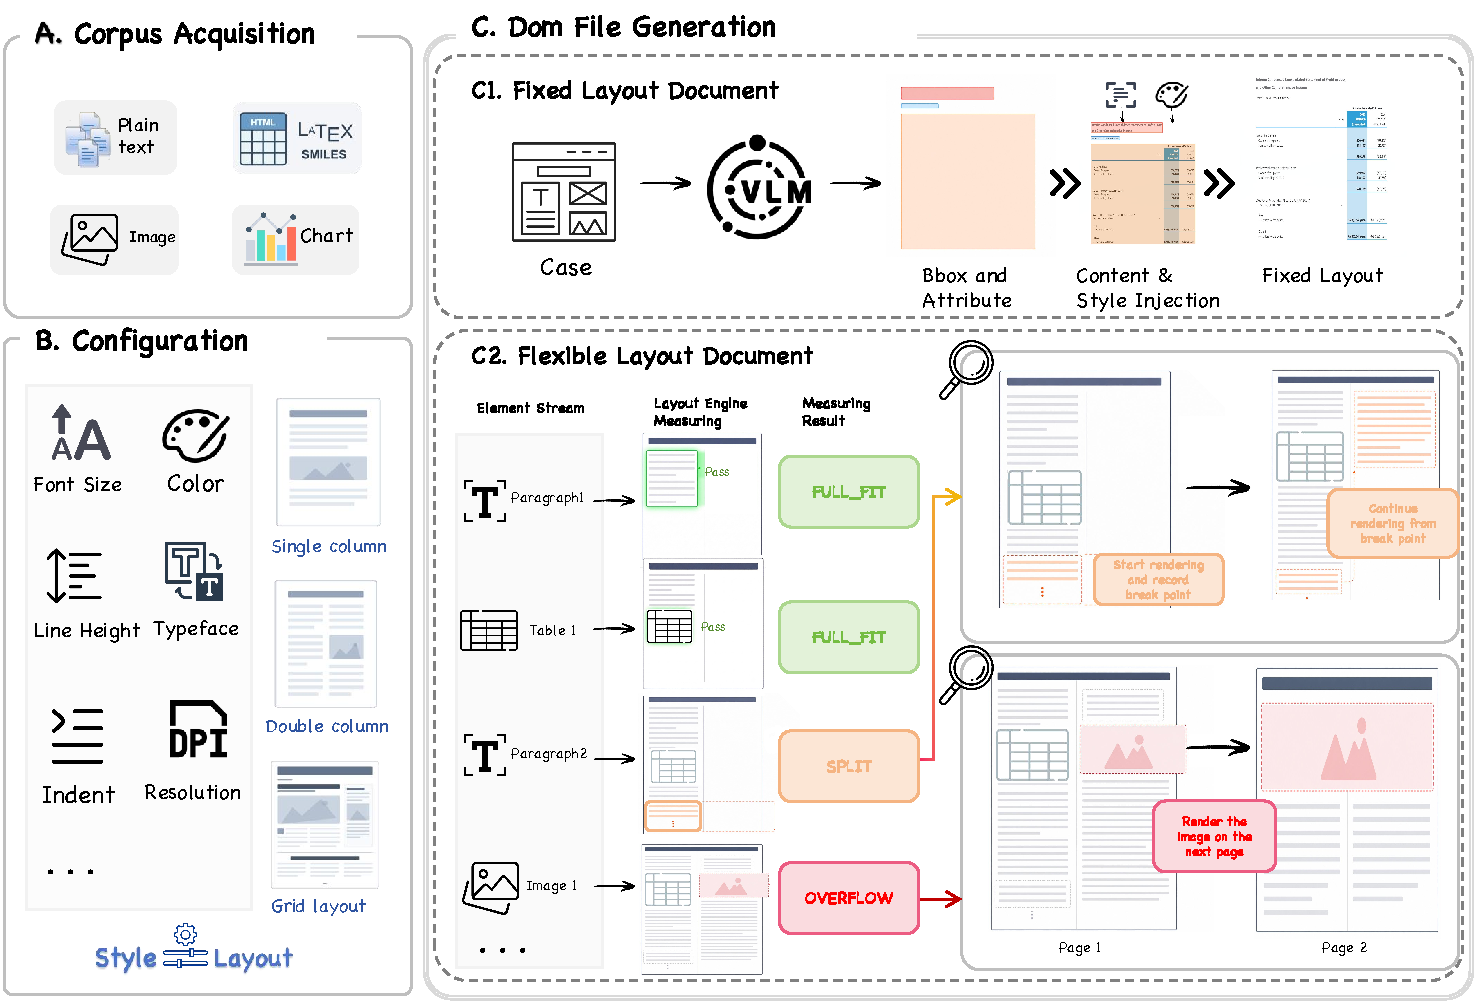
\includegraphics[width=\textwidth]{figures/data-engine-0704.pdf}
    \caption{Overall framework of our DOM-based document data synthesis engine. \textbf{(A)}~Corpus acquisition gathers plain text, structured elements, and visual assets. \textbf{(B)}~Configuration sets the page layout and element styles of a document template. \textbf{(C)}~DOM file generation instantiates documents along two paths. The fixed-layout path reproduces the layout of a real exemplar by vision-language parsing followed by content and style injection, while the flexible-layout path streams elements through a layout engine that measures each element and resolves it as \texttt{FULL\_FIT}, \texttt{SPLIT}, or \texttt{OVERFLOW} to produce content-elastic, multi-page layouts. Fine-grained labels are read directly off the laid-out DOM.}
    \label{fig:data_synth_engine}
\end{figure*}

\textbf{Corpus Acquisition.} This stage gathers the raw content (plain text, structured elements, and visual assets) that populates the synthetic documents. \textit{General text} comprises multilingual paragraphs drawn from public sources~\cite{wikimedia_dumps}, internal databases, and model distillation, filtered by length, language (English, Simplified Chinese, Traditional Chinese, etc.), and domain (academic, financial, educational, etc.) to match downstream document types. \textit{Structured elements} include tables, mathematical formulas, charts, and chemical formulas, represented as HTML, LaTeX, CSV, and SMILES strings collected from arXiv and public datasets~\cite{pubtabnet,unimernet,decimer}. \textit{Visual assets} consist of figures and images~\cite{ng2021understandingguidedimagecaptioning} embedded as document illustrations.

\textbf{Configuration.} A template defines the global appearance of a document through two complementary groups of parameters:

\begin{itemize}[leftmargin=1.0em, labelsep=0.5em]
    \item \textbf{Page-level parameters} govern the canvas and its functional regions: page size and margins, rendering resolution, the writing mode (horizontal or vertical) and text direction (left-to-right or right-to-left), the layout mode of the main body (single-column, multi-column, and grid layout), and the placement of auxiliary regions such as headers, footers, page numbers, and rotated side bars.
    \item \textbf{Element-level parameters} specify the visual style of each content type (body text, multi-level headings, ordered and unordered lists, tables, figures, inline and block equations, code, algorithms, and references), covering typography (font family and size, color, line height, alignment, indentation, and spacing) together with a block-flow attribute that determines how each block wraps and breaks across columns and pages.
\end{itemize}

Rather than fixing these parameters, each template stores a preset default value together with a small perturbation range for every parameter. At generation time, we jitter the defaults (font sizes, margins, line spacing, colors, and region geometry) within these bounds, so that a single template instantiates into a family of documents that share the same logical structure yet differ in fine-grained appearance. This turns every template into a source of controlled data augmentation, substantially enlarging visual diversity while keeping each layout typographically valid. Moreover, the perturbation ranges need not be uniform: when the engine is driven by our data flywheel (Sec.~\ref{sec:flywheel}), they can be biased toward the layout and document-type weaknesses recorded in its weakness taxonomy, so that augmentation concentrates on the regions where the parser currently underperforms. Maintaining a library of such templates across common document types (academic papers, financial reports, books, letters, and the like) lets the engine cover a broad space of real-world layouts.

\textbf{DOM File Generation.} Given the acquired corpus and a sampled template, this stage instantiates documents along two complementary paths. The \emph{fixed-layout} path targets document types whose visual form must closely match real specimens, such as financial reports and forms. It takes a real page as a layout exemplar, uses a vision-language model to recover its region bounding boxes and attributes, and injects sampled content and template styles into that layout, producing documents that preserve the exemplar's structure while varying its content. The \emph{flexible-layout} path instead composes each document from scratch, letting page count and element placement emerge from the content so as to cover a broad space of multi-column, multi-page layouts.

In the flexible-layout path, the engine first instantiates a complete DOM tree that serves as the document's logical intermediate representation. Every node is typed against a single element schema (paragraph, multi-level heading, list, table, figure, inline or block formula, code, header, footer, and side bar), and this type later drives renderer dispatch. The schema is open, so new modalities such as charts and chemical formulas are introduced by registering a node type and its renderer rather than by modifying the pipeline. Each node carries three pieces of information:
\begin{itemize}[leftmargin=1.0em, labelsep=0.5em]
    \item its \textbf{content}, retained in the native source form of each modality (plain text, LaTeX for formulas, HTML for tables, SMILES for molecules, etc.), so that nothing is lost to a lossy intermediate encoding.
    \item its \textbf{structural role} (heading level, reading order, and parent--child containment), which makes the document hierarchy explicit.
    \item a \textbf{style descriptor} sampled from the template (typography, alignment, spacing), together with a \emph{block-flow constraint} that declares how the node may be paginated: \emph{flexible} (freely splittable, e.g.\ body text, headings, and code), \emph{continuous} (splittable but order-preserving, e.g.\ tables and lists), or \emph{atomic} (indivisible, e.g.\ a figure and its caption).
\end{itemize}

Crucially, the DOM emitted at this point is purely \emph{logical}: it fixes content, hierarchy, and appearance but leaves all geometry unresolved, deferring coordinate computation to rendering, which repopulates the \emph{same} tree with exact positions. The DOM is thus a single source of truth from which one traversal yields ground-truth annotations for multiple downstream tasks: reading order, element-type and hierarchy labels, and structured text (Markdown/LaTeX/HTML) reconstructed directly from node content, without any additional labeling step. This explicit encoding of structural relations is precisely why we adopt a DOM rather than a flatter intermediate such as a Markdown or LaTeX string, from which hierarchy, reading order, and element boundaries would otherwise have to be recovered post hoc.

The flexible path then resolves this logical DOM into a concrete, paginated document, rasterizes it, and reads every label directly off the laid-out tree. Rather than \emph{predicting} positions, the engine delegates typesetting to a real browser layout engine and then \emph{reads back} exact coordinates, so that all geometric labels are correct \emph{by construction}. Three tightly coupled components carry out this rendering.

\textit{Layout planning.} The page canvas is first divided into functional regions (a main body together with headers, footers, and side bars), and the body is partitioned into a configurable arrangement of columns, rows, or grid cells, with cell extents taken from template ratios or jittered for diversity. The resulting regions are linearized into a reading sequence consistent with the document's writing mode (horizontal or vertical) and text direction (left-to-right or right-to-left), so that reading-order labels follow directly from the plan rather than being inferred from pixels.

\textit{Content-elastic pagination.} Elements are streamed into the planned regions one at a time, so that the page count emerges from the content itself rather than being fixed in advance. Before being committed, each element is rendered off-screen on a hidden measurement canvas and measured at its true rendered size, so that placement never relies on size estimates. Comparing this measured extent against the space left in the current region yields one of three outcomes (Figure~\ref{fig:data_synth_engine}). An element that fits entirely is placed in position (\texttt{FULL\_FIT}). An element that fits only partially is broken at a measured point and continues at the top of the next region, for instance the second column of the same page (\texttt{SPLIT}). An element that cannot be accommodated in the remaining space is deferred to the next region or page (\texttt{OVERFLOW}). How a block may be broken follows its block-flow constraint. \emph{Flexible} blocks break line by line across regions, \emph{continuous} blocks break while preserving order with table headers repeated on every continuation, and \emph{atomic} blocks are never broken. When an atomic block overflows, the engine performs a \emph{backward reflow}, either re-laying the most recently placed blocks to reclaim room on the current page or deferring the block to the next page, which removes orphaned fragments while preserving the global reading order.

\textit{Element pre-rendering.} Complex elements pass through dedicated sub-renderers \emph{before} measurement, so that their true footprint, rather than an approximation, drives layout. Formulas are typeset to SVG by a LaTeX engine and synchronized on web-font readiness, with display equations assigned document-global numbering. Tables are rendered from HTML/CSS inside an isolated shadow DOM, their logical cell grid (including row and column spans) recovered, and cross-page cut points located by binary search over measured geometry within the boundary cell, under typographic safeguards that forbid mid-word breaks, line-leading punctuation, and orphaned sub/superscripts. Images and custom fonts (CJK, Latin, and mixed scripts) are fully loaded before measurement to prevent reflow. Dispatch is keyed on element type and routed through a shared library manager, so the engine extends to additional notation renderers, such as charts and chemical formulas, by registering a renderer rather than altering the pipeline.

Finally, each laid-out page is rasterized at high resolution by device-pixel supersampling (optionally composited over template-controlled background textures for visual variability), and, in lockstep with the image, per-task labels are exported by traversing the laid-out DOM: character-, line-, and cell-level bounding boxes obtained from the browser's native geometry queries and offset into absolute page coordinates, alongside reading-order, element-type, hierarchy, and structured-text labels. Because the pixels and the annotations are read from one and the same DOM, they are exact and mutually consistent by construction, requiring no post-hoc detection or OCR.

% ============================================================
% Section 3: Dataset Preparation
% ============================================================
\subsection{Dataset Preparation}
\label{sec:dataset}

\begin{table*}[t]
\centering
\caption{Overview of the final training data composition of Infinity-Parser2. Sources span public datasets, flywheel-mined real documents, and synthesis-engine data. The original size denotes the total number of available samples, while the sampled size indicates the number retained after balanced sampling.}
\label{tab:dataset_summary}
\resizebox{\textwidth}{!}{%
\begin{tabular}{l|c|l|c|c}
\toprule
\textbf{Task} & \textbf{Sub-Task} & \textbf{Dataset} & \textbf{Original Size} & \textbf{Sampled Size} \\
\midrule
\multicolumn{5}{l}{\textit{Document Structure Tasks}} \\
\midrule
\multirow{5}{*}{Document Parsing}
  & \multirow{3}{*}{doc2json} & Pseudo-Labeled Web Documents & 776K & 776K\\
  &                           & Manually Labeled Newspaper               & 2.5K & 2.5K \\
  &                           & Synthesized Documents                             & 251K & 251K \\
\cmidrule(l){2-5}
  & \multirow{2}{*}{doc2md}   & Infinity-Doc-400K~\cite{wang2025infinity}    & 57K  & 57K \\
  &                           & Web-Crawled Handwritten Docs           & 62K  & 62K \\
\midrule
\multirow{2}{*}{Layout Analysis}
  & \multirow{2}{*}{layout\_analysis}       & M$^{6}$Doc~\cite{cheng2023m6doclargescalemultiformatmultitype} & 4K & 4K \\
  &                           & Synthesized Documents                             & 30K  & 30K \\
\midrule
\multicolumn{5}{l}{\textit{Element-level Parsing Tasks}} \\
\midrule
\multirow{3}{*}{Table Parsing}
  & table2html                & PubTabNet~\cite{pubtabnet}, FinTabNet~\cite{fintabnet}, MMTab-HTML~\cite{mmtab}             & 676K & 676K \\
\cmidrule(l){2-5}
  & \multirow{2}{*}{table2md} & MMTab-MD~\cite{mmtab}                                      & 27K  & 27K \\
  &                           & Synthesized Tables                             & 309K & 309K \\
\midrule
Math Formula Parsing & formula2latex & im2latex~\cite{im2latex}, UniMER~\cite{unimernet}, HME~\cite{hme100k}, CROHME~\cite{crohme}                       & 1.1M & 631K \\
\midrule
\multirow{3}{*}{Chart Parsing}
  & chart2table & ChartSFT~\cite{chartsft}, Chart-MoE~\cite{chartmoe}, UniChart~\cite{unichart}                             & 1.5M & 315K \\
  & chart2json  & Chart-MoE~\cite{chartmoe}, ChartQA~\cite{chartqa}                                        & 900K & 315K \\
  & chart2code  & ChartGen~\cite{chartgen}, Chart2Code~\cite{chart2code}, Chart-MoE~\cite{chartmoe}                           & 1.2M & 315K \\
\midrule
Chemical Formula Parsing & chem2smiles & Synthesized Chemical Formula Images & 5.9M & 315K \\
\midrule
\multicolumn{5}{l}{\textit{Reasoning and Generalization Tasks}} \\
\midrule
\multirow{2}{*}{Document VQA} & \multirow{2}{*}{docvqa} & DocVQA~\cite{docvqa}, ChartQA~\cite{chartqa}, AI2D~\cite{ai2d}, DocReason25K~\cite{docreason25k},& \multirow{2}{*}{1.6M} & \multirow{2}{*}{315K} \\
& & InfoVQA~\cite{infovqa}, DT-VQA~\cite{dtvqa}, TinyChart~\cite{tinychart} & & \\
\midrule
\multirow{2}{*}{General Multimodal Understanding} & \multirow{2}{*}{general\_mmu} & M4-Instruct~\cite{m4instruct}, LLaVA-v1.5~\cite{llava15}, ShareGPT-4V~\cite{sharegpt4v}, ShareGPT-4o~\cite{sharegpt4o}, CogVLM~\cite{cogvlm} & \multirow{2}{*}{3.2M} & \multirow{2}{*}{631K} \\
& & ALLaVA-Instruct~\cite{allava}, LVIS-Instruct~\cite{lvisinstruct4v}, TextVQA~\cite{textvqa}, OCRVQA~\cite{ocrvqa}, AnyWord-3M~\cite{anyword3m} & & \\
\midrule
\multicolumn{5}{l}{\textit{Others}} \\
\midrule
Blank-page Handling & - & Synthesized Documents & 5K & 5K \\
\bottomrule
\end{tabular}%
}
\end{table*}

This section describes the final training data composition of Infinity-Parser2, assembled after the data iteration flywheel (Sec.~\ref{sec:flywheel}) has converged. Each task draws from three sources: public datasets, real documents mined by the flywheel, and synthetic documents produced by the synthesis engine (Sec.~\ref{sec:synthesis}). For each task we report its definition, data sources, scale, annotation or synthesis strategy, and output format. A consolidated overview is given in Table~\ref{tab:dataset_summary}.

\textbf{Document Structure Tasks.} These tasks operate on the document as a whole and produce structural representations.

\begin{itemize}[leftmargin=1.0em, labelsep=0.5em]
    \item \textbf{Document Parsing.} Given an input document image, the model transforms it into a structured representation by identifying and ordering document elements according to the natural reading order, annotating each detected region with its element type, content, and spatial location, thereby converting unstructured pages into structured data. For the doc2json task, the training data combine real documents mined by the flywheel with synthetic documents produced by the synthesis engine: we mine 776K documents from the web spanning nine categories (exam papers, slides, academic papers, books, textbooks, magazines, notes, newspapers, and financial reports) and obtain high-quality pseudo labels for them through Stage 3 of our flywheel, manually annotate 2.5K complex newspaper images, and synthesize an additional 251K documents with our synthesis engine. For the doc2md task, we sample 57K high-quality examples from Infinity-Doc-400K~\cite{wang2025infinity} and mine 62K scanned handwritten image–text pairs from the Library of Congress digital archives.

    \item \textbf{Layout Analysis.} Layout analysis detects document elements in reading order and predicts their types and bounding boxes without recognizing their content. The training data comprise 4K samples from the publicly available M$^{6}$Doc dataset~\cite{cheng2023m6doclargescalemultiformatmultitype}, supplemented with 30K samples from our synthesis engine, for which layout labels are obtained directly from the DOM at near-zero cost. The outputs follow a standard layout-element schema covering titles, paragraphs, formulas, tables, figures, captions, headers, and footers.
\end{itemize}

\textbf{Element-level Parsing Tasks.} These tasks operate on individual document elements and produce element-specific content.

\begin{itemize}[leftmargin=1.0em, labelsep=0.5em]
    \item \textbf{Table Parsing.} Table parsing focuses on recognizing the content of table elements and producing structured sequences such as HTML and Markdown. For the table2html task, we collect 676K samples from PubTabNet~\cite{pubtabnet}, FinTabNet~\cite{fintabnet}, and MMTab-HTML~\cite{mmtab}. For the table2md task, we obtain 27K samples from MMTab-MD~\cite{mmtab} and generate an additional 309K samples with our synthesis engine.

    \item \textbf{Math Formula Parsing.} Math formula parsing recognizes the content of mathematical formula elements and produces structured LaTeX sequences. We collect 1.1M samples from im2latex~\cite{im2latex}, UniMER~\cite{unimernet}, HME~\cite{hme100k}, and CROHME~\cite{crohme}.

    \item \textbf{Chart Parsing.} Chart parsing converts visual charts (bar, line, pie, scatter, etc.) into structured data records and Python code. For the chart2table task, we collect 1.5M samples from ChartSFT~\cite{chartsft}, Chart-MoE~\cite{chartmoe}, and UniChart~\cite{unichart}. For the chart2json task, we obtain 900K samples from Chart-MoE~\cite{chartmoe} and ChartQA~\cite{chartqa}. For the chart2code task, we collect 1.2M samples from ChartGen~\cite{chartgen}, Chart2Code~\cite{chart2code}, and Chart-MoE~\cite{chartmoe}.

    \item \textbf{Chemical Formula Parsing.} Chemical formula parsing recognizes 2D chemical formula diagrams and outputs their SMILES representations. Because real-world annotated data are scarce, this task relies heavily on our synthesis engine, which renders chemical formulas from SMILES corpora into diagram images with controlled visual styles. Using four rendering backends (CDK~\cite{cdk}, RDKit~\cite{rdkit}, OpenChemLib~\cite{openchemlib}, and Indigo~\cite{indigo}) and a corpus drawn from DECIMER~\cite{decimer}, we generate 5.9M samples.
\end{itemize}

\textbf{Reasoning and Generalization Tasks.} These tasks go beyond per-element recognition and require document-level understanding or cross-domain generalization.

\begin{itemize}[leftmargin=1.0em, labelsep=0.5em]
    \item \textbf{Document VQA.} Document VQA requires answering natural-language questions grounded in a document image. We collect 1.6M samples from DocVQA~\cite{docvqa}, ChartQA~\cite{chartqa}, AI2D~\cite{ai2d}, DocReason25K~\cite{docreason25k}, InfoVQA~\cite{infovqa}, DT-VQA~\cite{dtvqa}, and TinyChart~\cite{tinychart}.

    \item \textbf{General Multimodal Understanding.} To preserve the open-domain vision-language alignment of the underlying VLM and mitigate catastrophic forgetting during document-heavy fine-tuning, we additionally include general image–text pairs and instruction data. In total, we collect 3.2M samples from public multimodal corpora, including M4-Instruct~\cite{m4instruct}, LLaVA-v1.5~\cite{llava15}, ShareGPT-4V~\cite{sharegpt4v}, ShareGPT-4o~\cite{sharegpt4o}, CogVLM~\cite{cogvlm}, ALLaVA-Instruct~\cite{allava}, LVIS-Instruct~\cite{lvisinstruct4v}, TextVQA~\cite{textvqa}, OCRVQA~\cite{ocrvqa}, and AnyWord-3M~\cite{anyword3m}.
\end{itemize}

\textbf{Blank-page Handling.} Beyond the task-specific data above, we additionally curate 5K blank-page samples spanning varying resolutions, background colors, and background textures. For inputs containing no valid content, the model is trained to emit task-specific empty outputs (e.g., empty Markdown, empty JSON array). This explicitly suppresses hallucinations on degenerate inputs and improves system robustness.

\textbf{Dataset Summary.} Overall, the final training set (Table~\ref{tab:dataset_summary}) combines public, flywheel-mined, and synthesis-engine data across structure-level, element-level, and reasoning tasks, comprising approximately 5M samples after balanced sampling. The sampling ratios are designed to ensure balanced coverage along the multi-attribute schema introduced in Sec.~\ref{sec:flywheel}, and to remain consistent with the bad-case distribution observed at flywheel convergence. To foster further progress in document parsing, after removing business-sensitive and privacy-related samples, we open-source the \textbf{Infinity-Doc2-5M} dataset at~\url{https://huggingface.co/datasets/infly/Infinity-Doc2-5M}.

\section{Model Training}

\begin{figure*}[htbp]
    \centering
    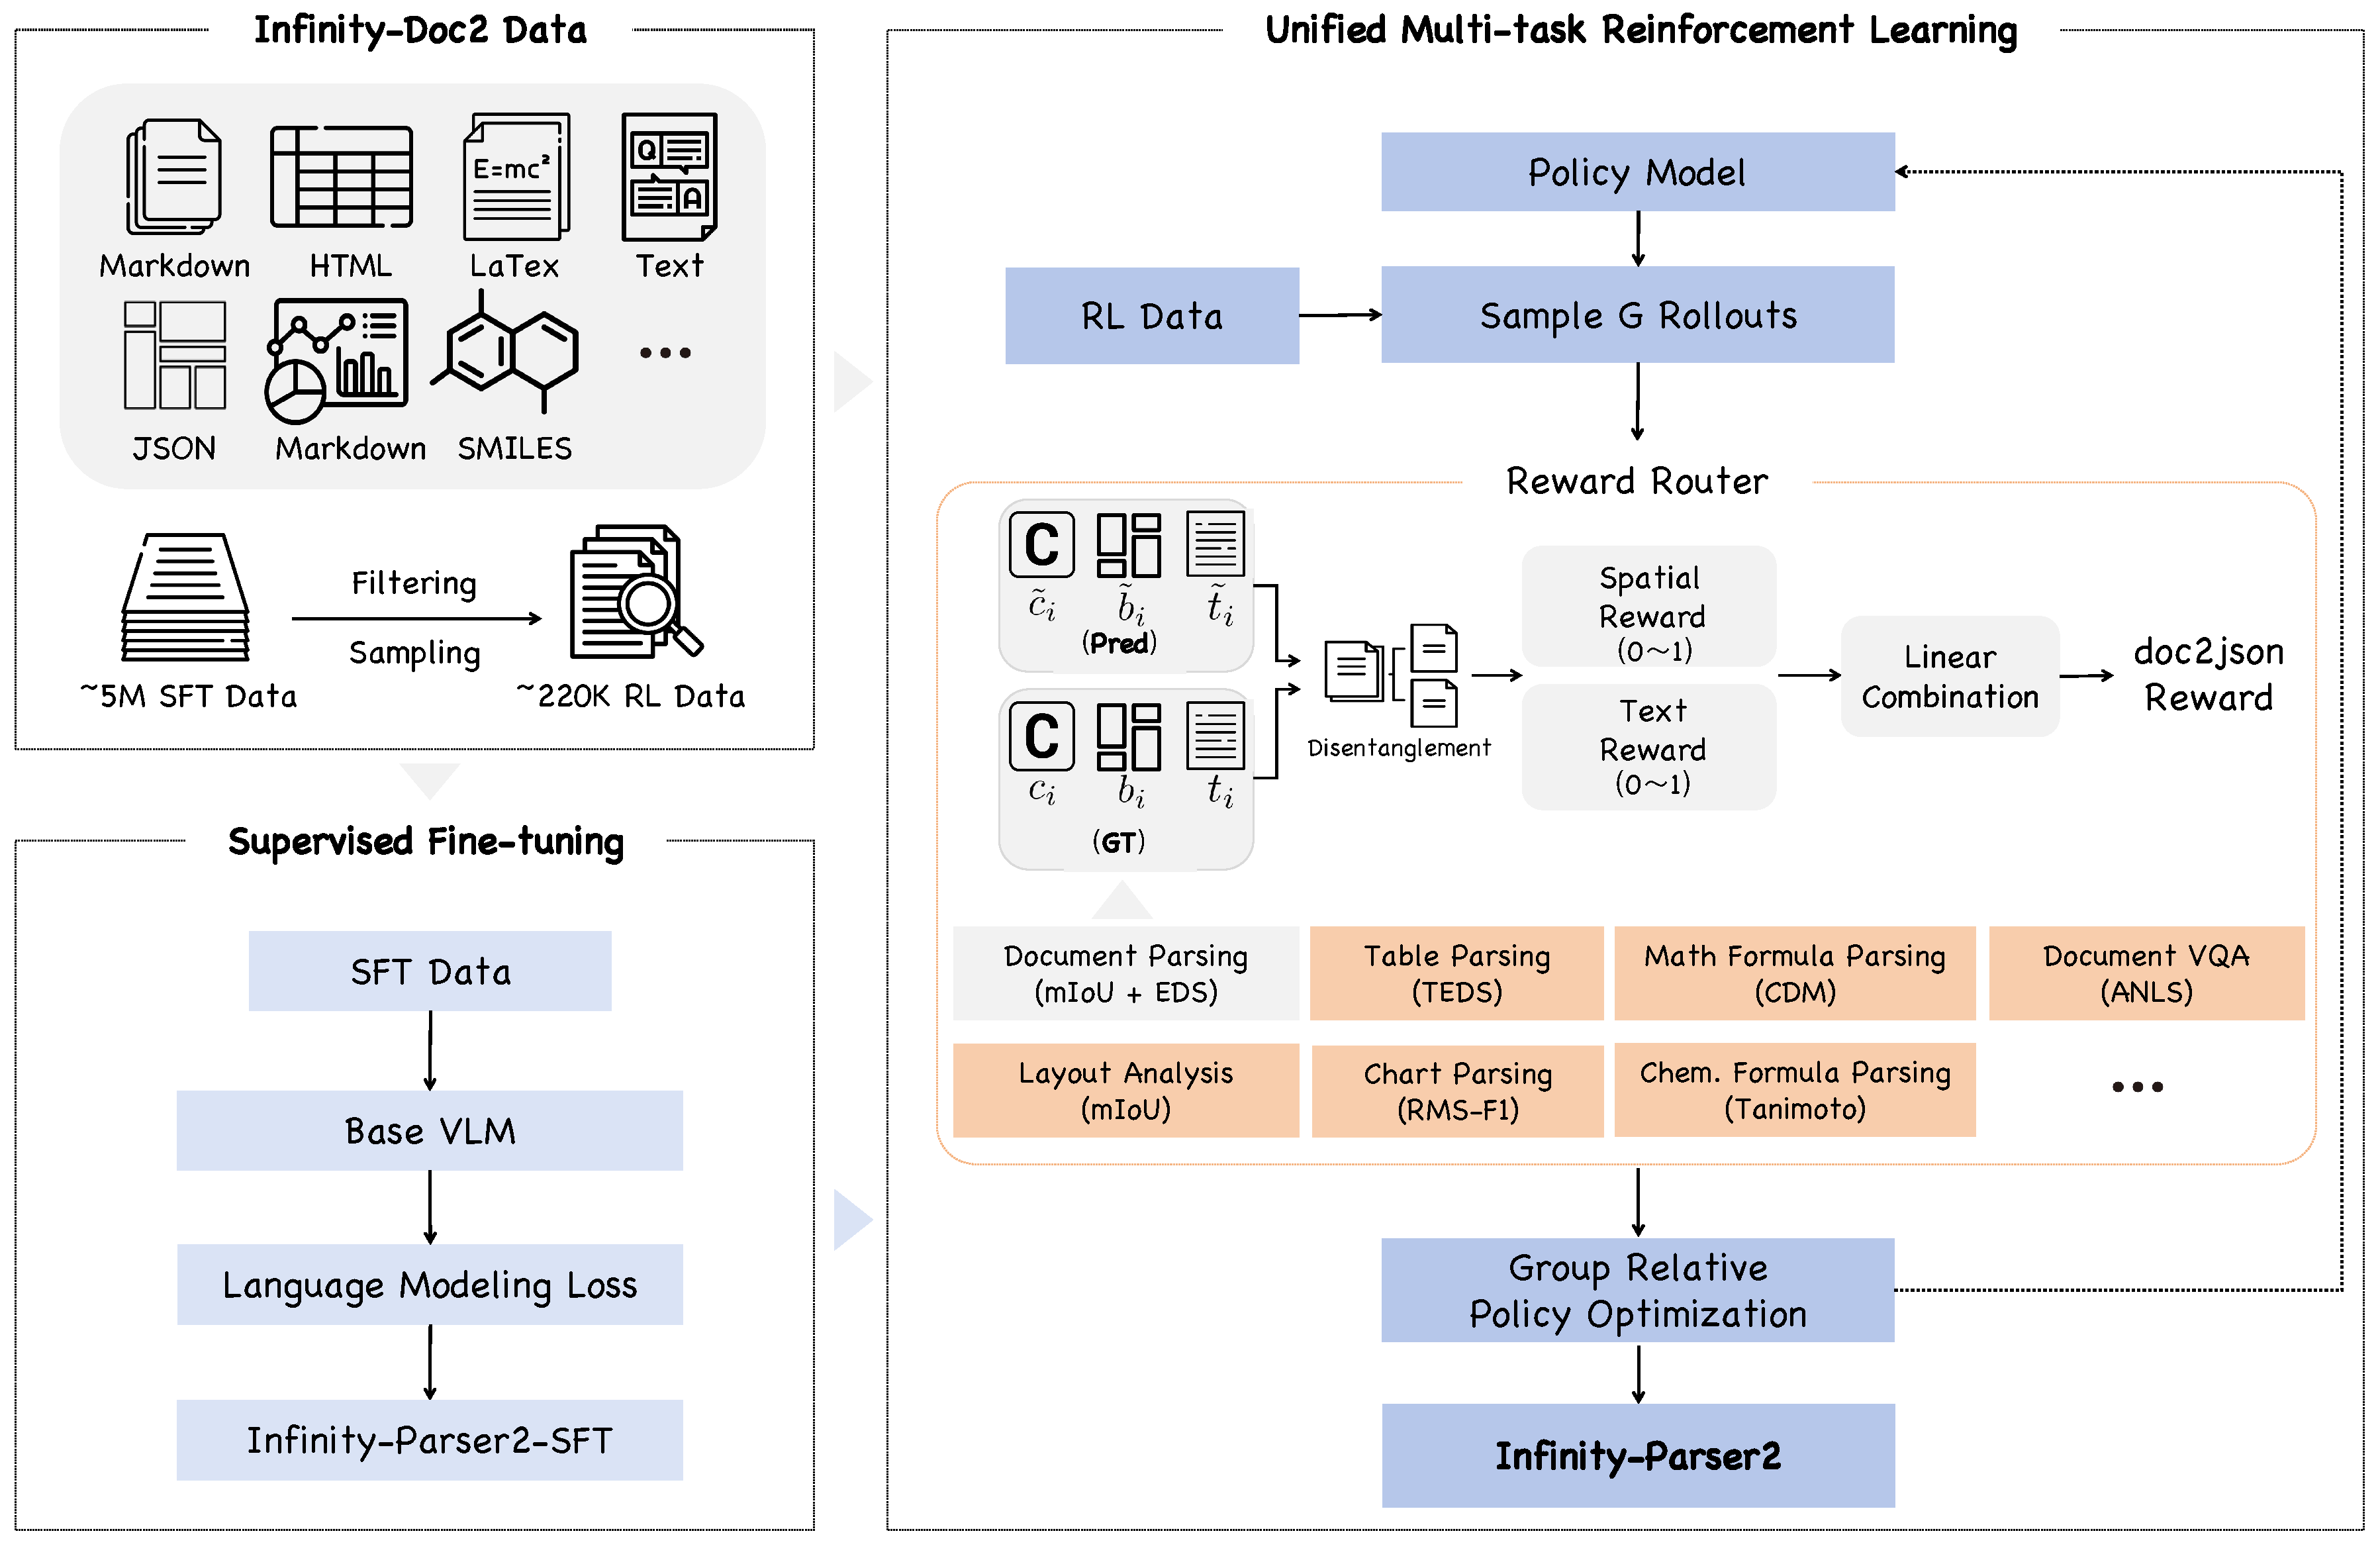
\includegraphics[width=\textwidth]{figures/overall_training_strategy_0707.pdf}
    \caption{Overall framework of Infinity-Parser2. We cast document parsing as a unified image-to-sequence problem: a single model maps a document image and a task instruction to a structured output (Markdown, HTML, LaTeX, JSON, etc.), with the target task selected solely by the instruction. Training proceeds in two stages, supervised fine-tuning (SFT) for broad multi-task parsing capability followed by joint reinforcement learning with verifiable rewards (RLVR) that co-trains all tasks under one policy, each rewarded by its own native evaluation metric.}
    \label{fig:overall_framework}
\end{figure*}

\subsection{Overall Training Strategy}

We formulate document parsing as a unified image-to-sequence generation problem. Given a document image $I$ and a task instruction $c$ that specifies the target task and output format, the model $\pi_\theta$ autoregressively generates a token sequence $y=(y_1,\dots,y_T)\sim\pi_\theta(\cdot\mid I,c)$ that decodes into a structured representation $[e_1,\dots,e_N]$, an ordered list of document elements rendered in Markdown, HTML, LaTeX, JSON, etc., where each $e_i$ carries the $i$-th element's type, content, and spatial location (where applicable). A single parameter set $\theta$ thus serves the entire parsing stack (document-, element-, and reasoning-level tasks) under one autoregressive interface, with the task selected solely through $c$.

As illustrated in Figure~\ref{fig:overall_framework}, training proceeds in two stages. We first perform supervised fine-tuning (SFT) to instill broad parsing capability through next-token prediction, and then conduct joint reinforcement learning with verifiable rewards (RLVR) to align the model with task-native evaluation metrics and to close the gap between teacher-forced training and autoregressive inference. This SFT-then-RLVR recipe follows recent document-parsing systems~\cite{wang2025infinity,poznanski2025olmocr2}. Our contribution lies in the design of the reward system that drives the RL stage rather than in the recipe itself. Concretely, our training design rests on three choices:

\begin{itemize}[leftmargin=1.0em, labelsep=0.5em]
    \item \textbf{Unified multi-task RLVR.} We co-train eight objectives (document parsing, layout analysis, table parsing, math formula parsing, chart parsing, chemical formula parsing, document VQA, and general multimodal understanding) within a single RL stage, rewarding each with a structure-aware metric native to that task (Sec.~\ref{sec:reward_design}).
    \item \textbf{Disentangled spatial--textual reward.} For structured-layout parsing, we introduce a reward that scores element localization and content fidelity separately, a signal absent from prior edit-distance- or unit-test-based rewards (Sec.~\ref{sec:str}).
    \item \textbf{Reward routing with normalization.} All objectives are optimized jointly through per-task reward routing and cross-task reward normalization, so that a single policy is trained over heterogeneous tasks with comparable gradient scales (Sec.~\ref{sec:rl_opt}).
\end{itemize}

Under this recipe we train two deployable variants on a shared architecture (Infinity-Parser2-Flash for low-latency inference and Infinity-Parser2-Pro for precision-critical settings), whose configurations are detailed in our experimental setup.

\subsection{Supervised Fine-Tuning}
\label{sec:sft}

We adopt Qwen3.5~\cite{qwen3.5} as our foundation model, a vision--language model pre-trained on large-scale multimodal data with strong inherent document-understanding capability. We fine-tune it on Infinity-Doc2-5M (Sec.~\ref{sec:dataset}) with a supervised next-token-prediction objective:
\begin{equation}
\mathcal{L}_{\mathrm{SFT}}(\theta) = -\,\mathbb{E}_{(I,c,y)\sim\mathcal{D}}\sum_{t=1}^{|y|}\log\pi_\theta\!\left(y_t \mid y_{<t}, I, c\right),
\end{equation}
where $\mathcal{D}$ denotes the training corpus and each triple $(I,c,y)$ pairs an input image and task instruction with its target sequence. The SFT corpus spans all sub-tasks, including the full general-multimodal-understanding set, which preserves the open-domain vision--language alignment of the base model and mitigates catastrophic forgetting during document-heavy fine-tuning. This stage endows the model with broad multi-task parsing competence and provides a strong initialization for the subsequent RL stage.

\subsection{Joint Reinforcement Learning with Verifiable Rewards}
\label{sec:reinforcement_learning}

\subsubsection{Motivation}

The next-token-prediction objective of SFT, trained with teacher forcing, optimizes the model under a ground-truth-conditioned distribution that differs from the autoregressive distribution encountered at inference. This exposure bias encourages the model to overfit the sequential dependencies and annotation noise of the training data, limiting its generalization to unseen document types. To bridge this train--inference gap, we add a reinforcement learning stage in which the model generates full sequences (rollouts) and is optimized against task-specific reward signals, promoting robust generation strategies that transfer better to out-of-distribution document formats. The effectiveness of this stage hinges entirely on the reward signals, whose design we describe next.

\subsubsection{Reward Design}
\label{sec:reward_design}

All RL signals in Infinity-Parser2 are \emph{verifiable rewards}: each is computed by a deterministic, reference-based metric rather than a learned reward model, which keeps the signal faithful to ground truth and structurally limits reward hacking. We adopt a single guiding principle, \emph{metric-as-reward}, under which every task is rewarded by its own native evaluation metric, so that RL optimizes directly for the quantity by which the task is ultimately judged. All rewards are normalized to $[0,1]$ to keep gradient magnitudes comparable across co-trained tasks (Sec.~\ref{sec:rl_opt}). When an output jointly encodes multiple facets (most notably structured-layout parsing, which couples element localization with textual content), a single scalar metric cannot separate distinct error modes. We therefore factorize the reward into facet-specific terms, as detailed below.

\paragraph{Disentangled Spatial--Textual Reward for Structured Parsing.}
\label{sec:str}
The doc2json task produces a joint detection--recognition structure: an ordered list of elements $E_i=(c_i,b_i,t_i)$, each carrying a category $c_i$, a bounding box $b_i$, and textual content $t_i$. Scoring such an output with a single edit distance over its serialized form is ill-suited on two counts: it conflates \emph{where} an element is with \emph{what} it contains, yielding an ambiguous learning signal, and it measures geometric error through coordinate digit strings, where a few-pixel shift can perturb the reward disproportionately. We therefore disentangle the reward into a spatial term and a textual term, each evaluated in its native space.

\textit{Spatial reward.} Matching predicted boxes to references requires a fragile assignment step (e.g., Hungarian matching) under an IoU threshold, and it further breaks down when the two sides are annotated at inconsistent granularity: a single reference block may be predicted as several finer boxes (one-to-N), or several reference blocks may be covered by one prediction (N-to-one), leaving no unambiguous one-to-one correspondence. We therefore avoid box matching altogether and instead score localization at the level of per-category occupied area. For each category $k$, we merge all predicted boxes of that category into a single region $P^{k}$ by geometric union, and likewise form $G^{k}$ from the references. The spatial reward is the mean area Intersection-over-Union (mIoU)~\cite{chen2018encoder} over the categories that appear in the prediction or the reference, $K=K_{\mathrm{pred}}\cup K_{\mathrm{gt}}$:
\begin{equation}
r_{\mathrm{spatial}} = \frac{1}{\lvert K\rvert}\sum_{k\in K}\frac{\lvert P^{k}\cap G^{k}\rvert}{\lvert P^{k}\cup G^{k}\rvert},
\end{equation}
where $\lvert\cdot\rvert$ denotes area and $\lvert K\rvert$ the number of categories. A category present on only one side has an empty intersection and thus contributes $0$. The unions and intersections are evaluated exactly from the box geometry, so the spatial reward requires no rasterization or resolution parameter. This region-overlap formulation is \emph{assignment-free} and \emph{order-invariant} at the box level, and remains robust to mis-counting: spurious predictions enlarge the union while missed regions shrink the intersection, both lowering the score without any explicit box matching.

\textit{Textual reward.} The element contents are concatenated in the predicted reading order into a single Markdown string $s_{\mathrm{pred}}$ and scored against the reference $s_{\mathrm{gt}}$ by Edit Distance Similarity, $r_{\mathrm{text}}=\mathrm{EDS}(s_{\mathrm{pred}},s_{\mathrm{gt}})$. Because the concatenation follows reading order, this term additionally penalizes reading-order errors, so localization, content fidelity, and reading order are jointly covered by the two terms without a dedicated ordering reward. Using EDS also keeps the content signal consistent with the doc2md task.

\textit{Combination.} The two terms are linearly combined,
\begin{equation}
r_{\mathrm{doc2json}} = \lambda\,r_{\mathrm{spatial}} + (1-\lambda)\,r_{\mathrm{text}},
\end{equation}
with both components in $[0,1]$. We report the weight $\lambda$ in our experimental setup. Predictions that cannot be parsed into the element list receive zero reward. Unlike prior RLVR-based parsers that reward only flat textual output (Infinity-Parser~\cite{wang2025infinity} couples edit distance with paragraph-count and reading-order terms but supplies no localization signal, while olmOCR-2~\cite{poznanski2025olmocr2} scores unit tests on rendered text rather than on coordinate-bearing structured output), this reward acts directly on the structured prediction, separately crediting \emph{where} each element is and \emph{what} it contains.

\paragraph{Reward Suite over the Co-trained Objectives.}
We extend the same metric-as-reward principle across all eight co-trained objectives:
\begin{itemize}[leftmargin=1.0em, labelsep=0.5em]
    \item \textbf{Document parsing.} doc2md is rewarded by EDS and doc2json by the spatial--textual reward above.
    \item \textbf{Layout analysis.} Layout analysis, which predicts typed boxes without content, is rewarded by the spatial term $r_{\mathrm{spatial}}$ alone.
    \item \textbf{Table parsing.} We use the Tree-Edit-Distance-based Similarity (TEDS)~\cite{zhong2020image} for both table2html and table2md, reflecting the hierarchical structure of tables.
    \item \textbf{Math formula parsing.} We use the Character Detection Matching (CDM) metric~\cite{wang2025imagetexttransformingformula} for formula2latex, which compares rendered formulas and is therefore robust to syntactically different but visually equivalent LaTeX.
    \item \textbf{Chart parsing.} We adopt the Relative Mapping Similarity F1 (RMS-F1)~\cite{liu2023deplot} for chart2table, the mean Average Precision from the Structuring Chart-oriented Representation Metric (SCRM)~\cite{xia2023structchart} for chart2json, and EDS for chart2code, treating the generated plotting code as a string.
    \item \textbf{Chemical formula parsing.} For chem2smiles we use the Tanimoto similarity~\cite{tanimoto1958elementary} between the predicted and reference molecular fingerprints.
    \item \textbf{Document VQA.} For docvqa we use the Average Normalized Levenshtein Similarity (ANLS).
    \item \textbf{General multimodal understanding.} We apply RLVR only to the verifiable subset of this objective (samples that carry reference short answers), scored by ANLS. Open-ended samples are excluded from RL and retained only in SFT.
\end{itemize}

\subsubsection{Optimization}
\label{sec:rl_opt}

We optimize the policy with Group Relative Policy Optimization (GRPO)~\cite{shao2024deepseekmathpushinglimitsmathematical}, which dispenses with a learned value model. For each input $(I,c)$, the current policy samples a group of $G$ rollouts $\{y^{(i)}\}_{i=1}^{G}$, each scored by its task reward $r^{(i)}\in[0,1]$. The group-relative advantage is obtained by normalizing rewards within the group,
\begin{equation}
\hat{A}^{(i)} = \frac{r^{(i)} - \mathrm{mean}\big(\{r^{(j)}\}_{j=1}^{G}\big)}{\mathrm{std}\big(\{r^{(j)}\}_{j=1}^{G}\big)}.
\end{equation}
The policy is then updated by maximizing the standard PPO-style clipped surrogate with these advantages, regularized by a KL penalty toward a frozen reference policy. Because every reward is verifiable, the advantage reflects genuine task quality rather than a learned proxy.

To co-train heterogeneous tasks in a single run, a \emph{reward router} dispatches each rollout to the reward function of its task, while the within-group normalization places all rewards on a common $[0,1]$ scale, keeping advantages comparable across tasks within a mixed batch. The RL training set is constructed by randomly sampling 5\% of each task from Infinity-Doc2-5M, yielding roughly 220K examples. Its detailed composition and the optimization hyperparameters are reported in our experimental setup.
